% !TeX root = ..\literaturereview.tex

\section{Deep learning}

\subsection{Machine learning}

We are in an age where there is so much data that in many cases, hand building a model to analyse, find patterns in and draw conclusions from the data is unfeasible, and so we use computers to analyse it in a process called \qt{Machine Learning} (ML)~\autocite[1]{murphy2012}.
Computers are able to do these tasks by combining information in nonlinear ways, but become more powerful when the output of one nonlinear process is fed into another nonlinear process, abstracting the raw data to a higher level.
\qtc[436]{lecun2015}{With the composition of enough such transformations, very complex functions can be learned}.

\subsubsection{Types of learning}

In \qt{unsupervised learning}, the algorithm is given only input data and its goal is to learn the patterns that make up the raw data.
This is most commonly used for cluster analysis, where the goal is to group unlabelled datapoints in a way that points with similar properties are in the same class.
For example, in market basket analysis, an ML algorithm will analyse the items in a customer's online basket and suggest similar products that the customer is likely to buy.

In \qt{supervised learning}, the algorithm is given a \qt{training set} of inputs and their corresponding outputs.
An error score is calculated to evaluate the success of the predictions, which the algorithm tries to minimise~\autocite[436]{lecun2015}.
The model learns the patterns of the training data, and then tries to predict the outcomes of some unseen \qt{test set} which checks if the algorithm has merely \qt{memorised} the patterns or if it has discovered some underlying structure in the data~\autocite[463--467]{lecun2015}.

A compromise between these two methods is \qt{semi-supervised learning} (or \qt{partially supervised learning}), where there is a high cost of labelling the training set, so only a portion of the data are labelled.
This is used in areas such as object recognition, where a human must label the objects at first, but once the algorithm can reliably identify objects in the images, it can become unsupervised.

Another very different type of learning is \qt{reinforcement learning}, where the algorithm is an agent that must decide on actions to take without knowing the consequences.
It receives a reward or loss based on its actions, and then updates its future decisions accordingly~\autocite[2]{alom2018}.
An example might be a robot navigating a maze.
It takes a loss for touching hazards and is rewarded for reaching a target location.
The key differences with this method are that the algorithm cannot directly see the function it is trying to optimise, and any action it takes will change its state.

\subsubsection{Types of prediction}

Supervised ML has two common prediction types: regression, where the outputs are continuous values; and classification, where the aim is to correctly assign the points to classes.
Classification can either involve predicting the most likely class for a datapoint or estimating the probability of being in each class, which is equivalent to regression of \(y_1, y_2, \dots, y_n\), where \(y_i \in [0, 1]\) is the probability of being in class \(i\).

\subsection{The neuron}

In 1957, psychologist Frank Rosenblatt proposed a stochastic electronic brain model, which he called a \qt{perceptron}~\autocite{rosenblatt1957}.
At the time, most models of the brain were deterministic algorithms which could recreate a single neural phenomenon such as memorisation or object recognition.
Rosenblatt's biggest criticism of these models was that while a deterministic algorithm could perform a single task perfectly, unlike a biological brain, it could not be generalised to perform many tasks without a lot of substantial changes.
He described deterministic models of the brain as \qtc[387]{rosenblatt1958}{amount[ing] simply to logical contrivances for performing particular algorithms \cut{} in response to sequences of stimuli}.
Another way he wanted his synthetic brain to mirror biological brains was the property of redundancy, the ability to have pieces removed and still function, which is not possible for deterministic algorithms where even a small change to a circuit or a line of code can stop all functionality.
It was a commonly held belief that deterministic algorithms \qtc[387]{rosenblatt1958}{would require only a refinement or modification of existing principles}, but Rosenblatt questioned this idea, believing that the problem needed a more fundamental re-evaluation.
At the heart of his idea was the \qt{perceptron}, which could -- through repeated training and testing -- receive a set of inputs and reliably give a correct binary response.
The perceptron was later generalised to the concept of an \qt{(artificial) neuron} (also called a \qt{unit}), which, instead of only giving a binary output, maps a finite number of real inputs to a single real output value.

Since the invention of \citeauthor{rosenblatt1957}'s perceptron, there have been many alternative models for neurons proposed, including fuzzy neurons, which allow truth values to be on a scale rather than a Boolean value~\autocite{gupta1991}; higher order neurons, which include second or higher products of the inputs~\autocite{rumelhart1986} and spiking neural networks, which use differential equations to emulate the electrical charge of biological neurons~\autocite{maass1997}.
We will only consider the simple neuron based on Rosenblatt's perceptron.

A neuron is defined by its weight vector~\(\vec{w}\), its bias~\(b\) and its activation function~\(\phi(\x)\).

The stages of a neuron, seen in Figure~\ref{neuron} are:
\begin{enumerate}
 \item For an input vector \(\vec{x} \in \reals^n\) and a weight vector \(\vec{w} \in \reals^n\), take a weighted sum of the inputs, called a \qt{linear combiner}.
       \[ \text{linear combiner} = \sum_{i=1}^{n}{x_i w_i} \]
 \item Then, a bias \(b \in \reals{}\) is added, which translates the output to a suitable range, called the pre-activation \((v)\).
       The importance of adding a bias is most clearly seen in the design of Rosenblatt's original perceptron using electronic circuitry, where a positive pre-activation would induce a current in the output wire, and a negative output would not.
       The bias controls how large the weighted sum needs to be to \qt{activate} the neuron.
       \[ \text{pre-activation} = v = \sum_{i=1}^{n}{x_i w_i} + b \]
 \item Finally, an \qt{activation function} (or \qt{limiter function}) \(\phi(\x)\) is applied, which restricts the output to a range and introduces nonlinearity to the system.
       As mentioned, Rosenblatt's perceptrons used the \(\operatorname{sign}(\x)\) function, which is now only used for binary classification problems.
       It is not useful for connecting to another neuron, as information about the magnitude of the output is lost.
       Commonly the sigmoid function \(S(x) = (1+\exp(-x))^{-1}\), the \(\tanh(\x)\) function or the \qt{softmax} function (a generalisation of the logistic function to vectors) are used.
       The most commonly used activation function for deep learning (see Section~\ref{deeplearning}) is the \ac{ReLU} function~\autocite{ramachandran2017}, which is defined as the positive part of its input \(\operatorname{ReLU}(x) = \max(0, x)\).
       If the activation function is the identity function, then optimising a neuron is equivalent to performing linear regression.
       The activation function must be differentiable if the gradient descent method is used (see Section~\ref{backpropagation}) as gradient descent relies on calculating the gradient of the error.
       \[ \text{neuron output} = y = \phi\left(\sum_{i=1}^{n}{x_i w_i} + b \right) \]
\end{enumerate}

\begin{figure}[htbp]
 \centering
 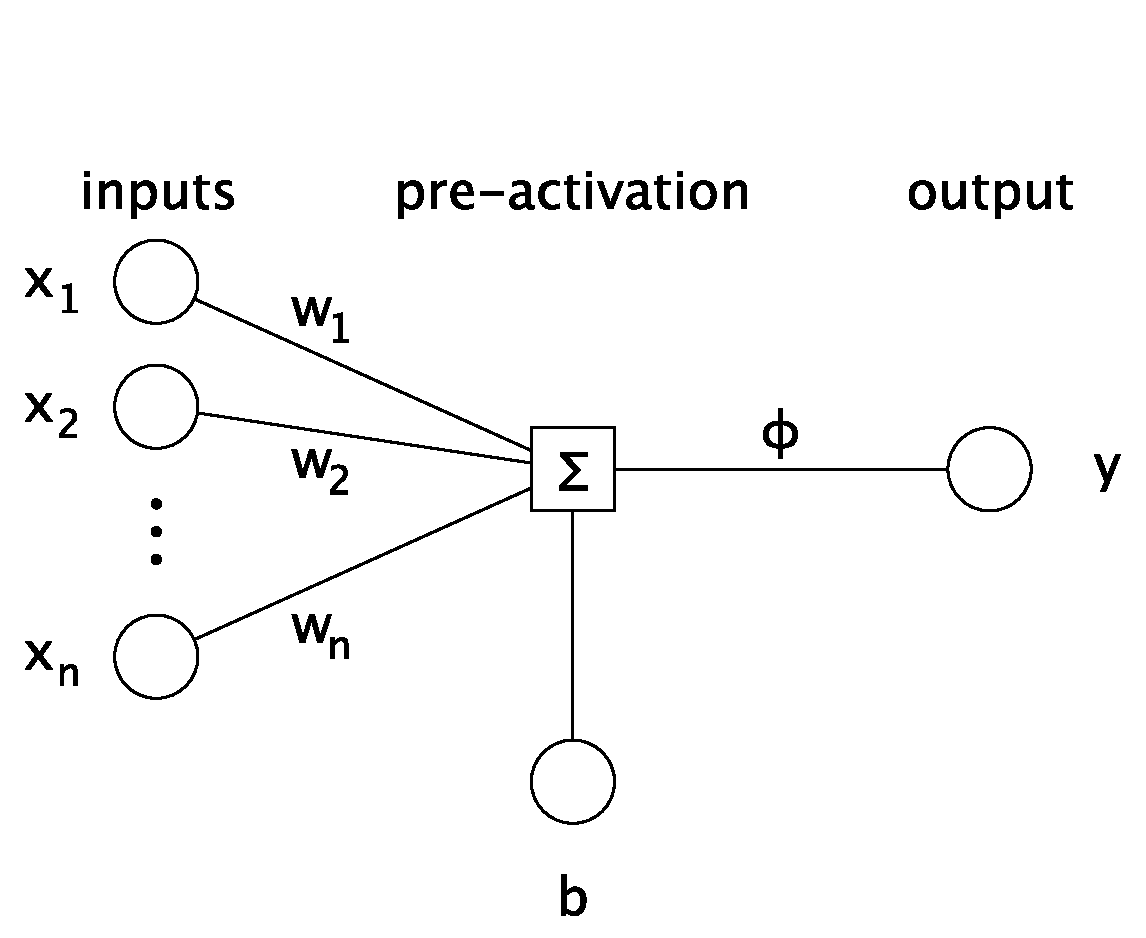
\includegraphics[width=1\textwidth]{neuron.pdf}
 \caption{A diagram of the steps in a neuron.}
 \label{neuron}
\end{figure}

\subsection{Artificial neural networks}

While a single perceptron can solve simple tasks, they become much more effective when connected together in a \qt{neural network} (or \ac{ANN}).
We will only consider \qt{feedforward neural networks}, where the neurons are connected in layers.
The first and last layers are known as the input and output layers respectively, and the layers in between are called \qt{hidden layers}.
In feedforward networks such as Figure~\ref{nnstructure}, the neurons on each layer are only connected to the neurons on adjacent layers and are not connected to each other.
This means information is passed through the network sequentially, as opposed to designs such as \qt{recurrent neural networks}, where the information is recursively passed in a loop before being output.

\begin{figure}[htbp]
 \centering
 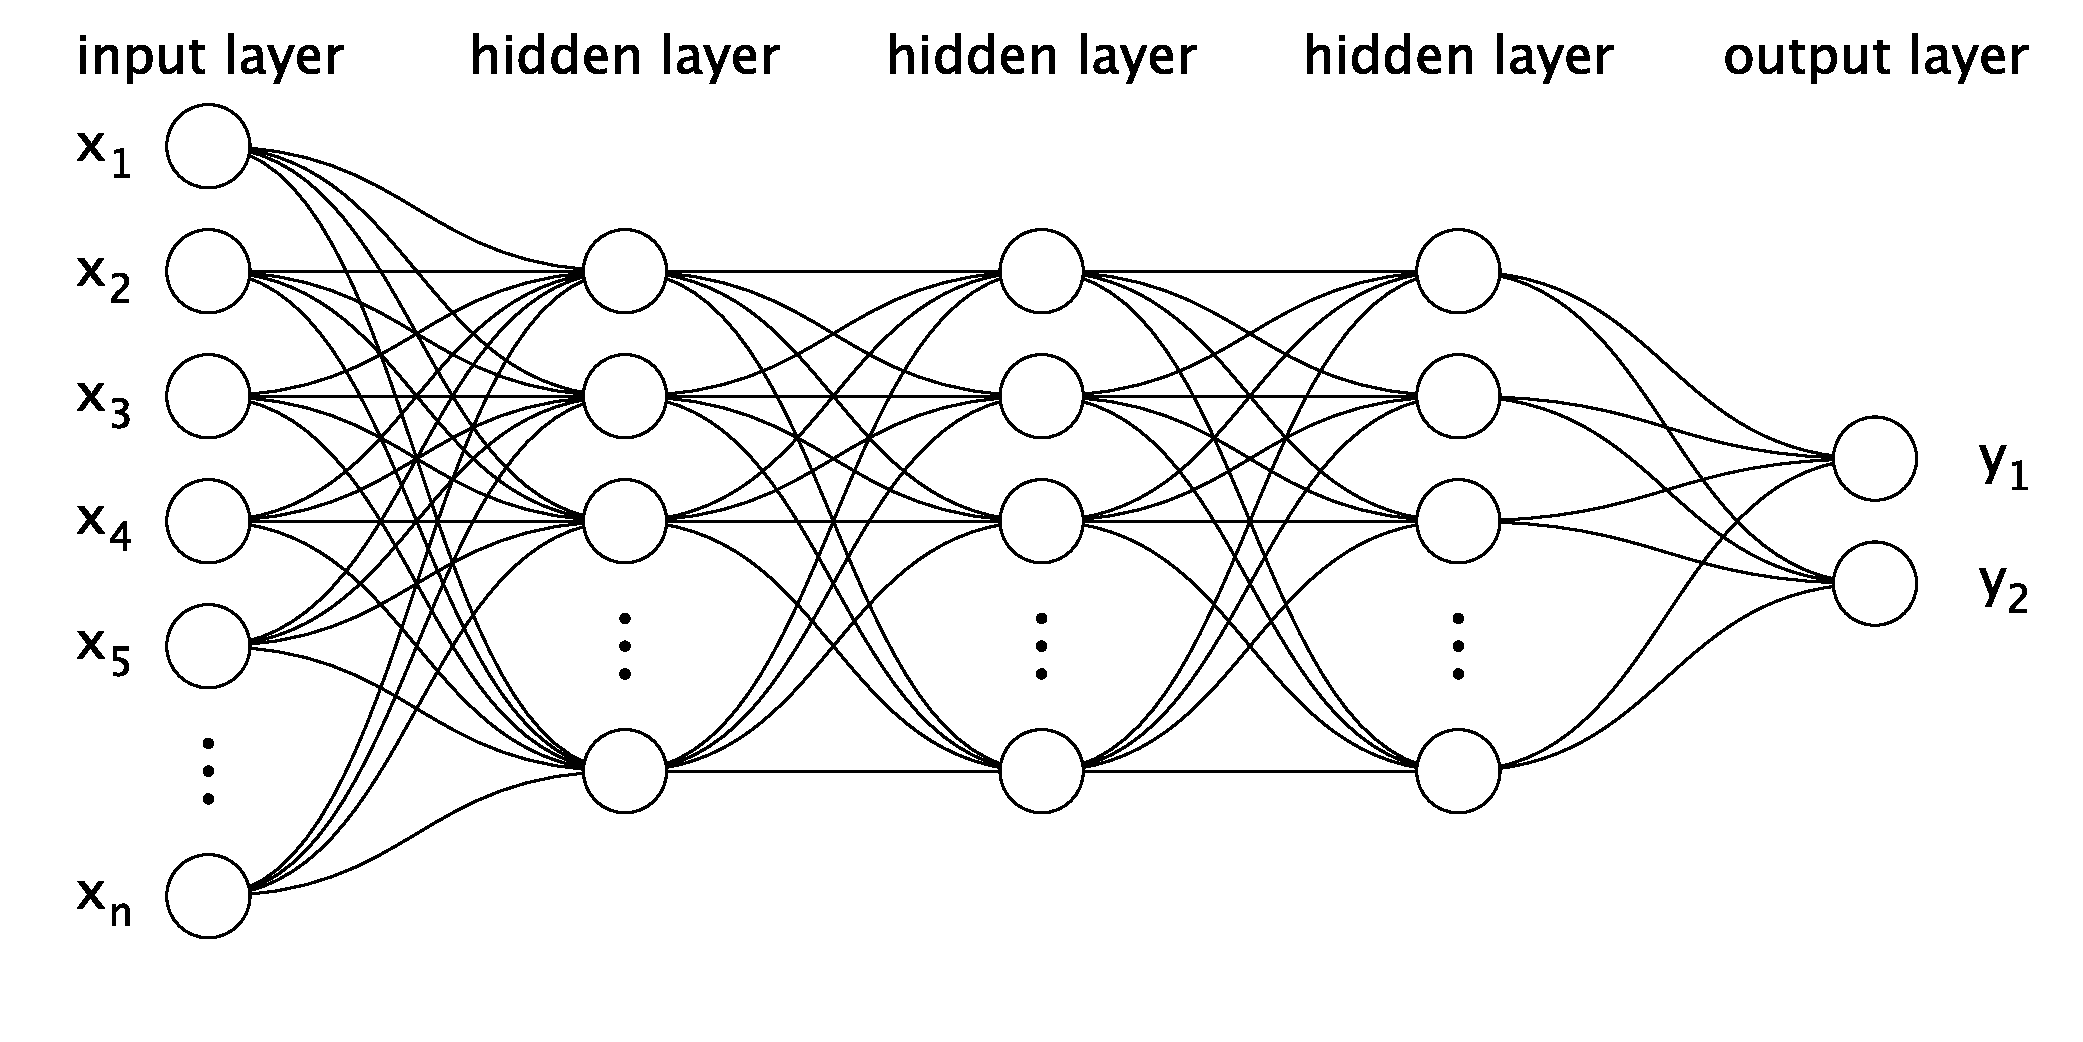
\includegraphics[width=\textwidth]{nnstructure.pdf}
 \caption{An example of a neural network's structure with \(n\) inputs and two outputs.}
 \label{nnstructure}
\end{figure}

\subsection{The backpropagation algorithm}\label{backpropagation}

Even in a small neural network like in Figure~\ref{examplenn}, there are more than 60 weights and biases which need to be tuned to produce accurate predictions.
A method to automatically optimise this was not understood until the 1980s, when the \qt{backpropagation} algorithm was independently discovered by \textcite{rumelhart1986a} among others.

\begin{figure}[htbp]
 \centering
 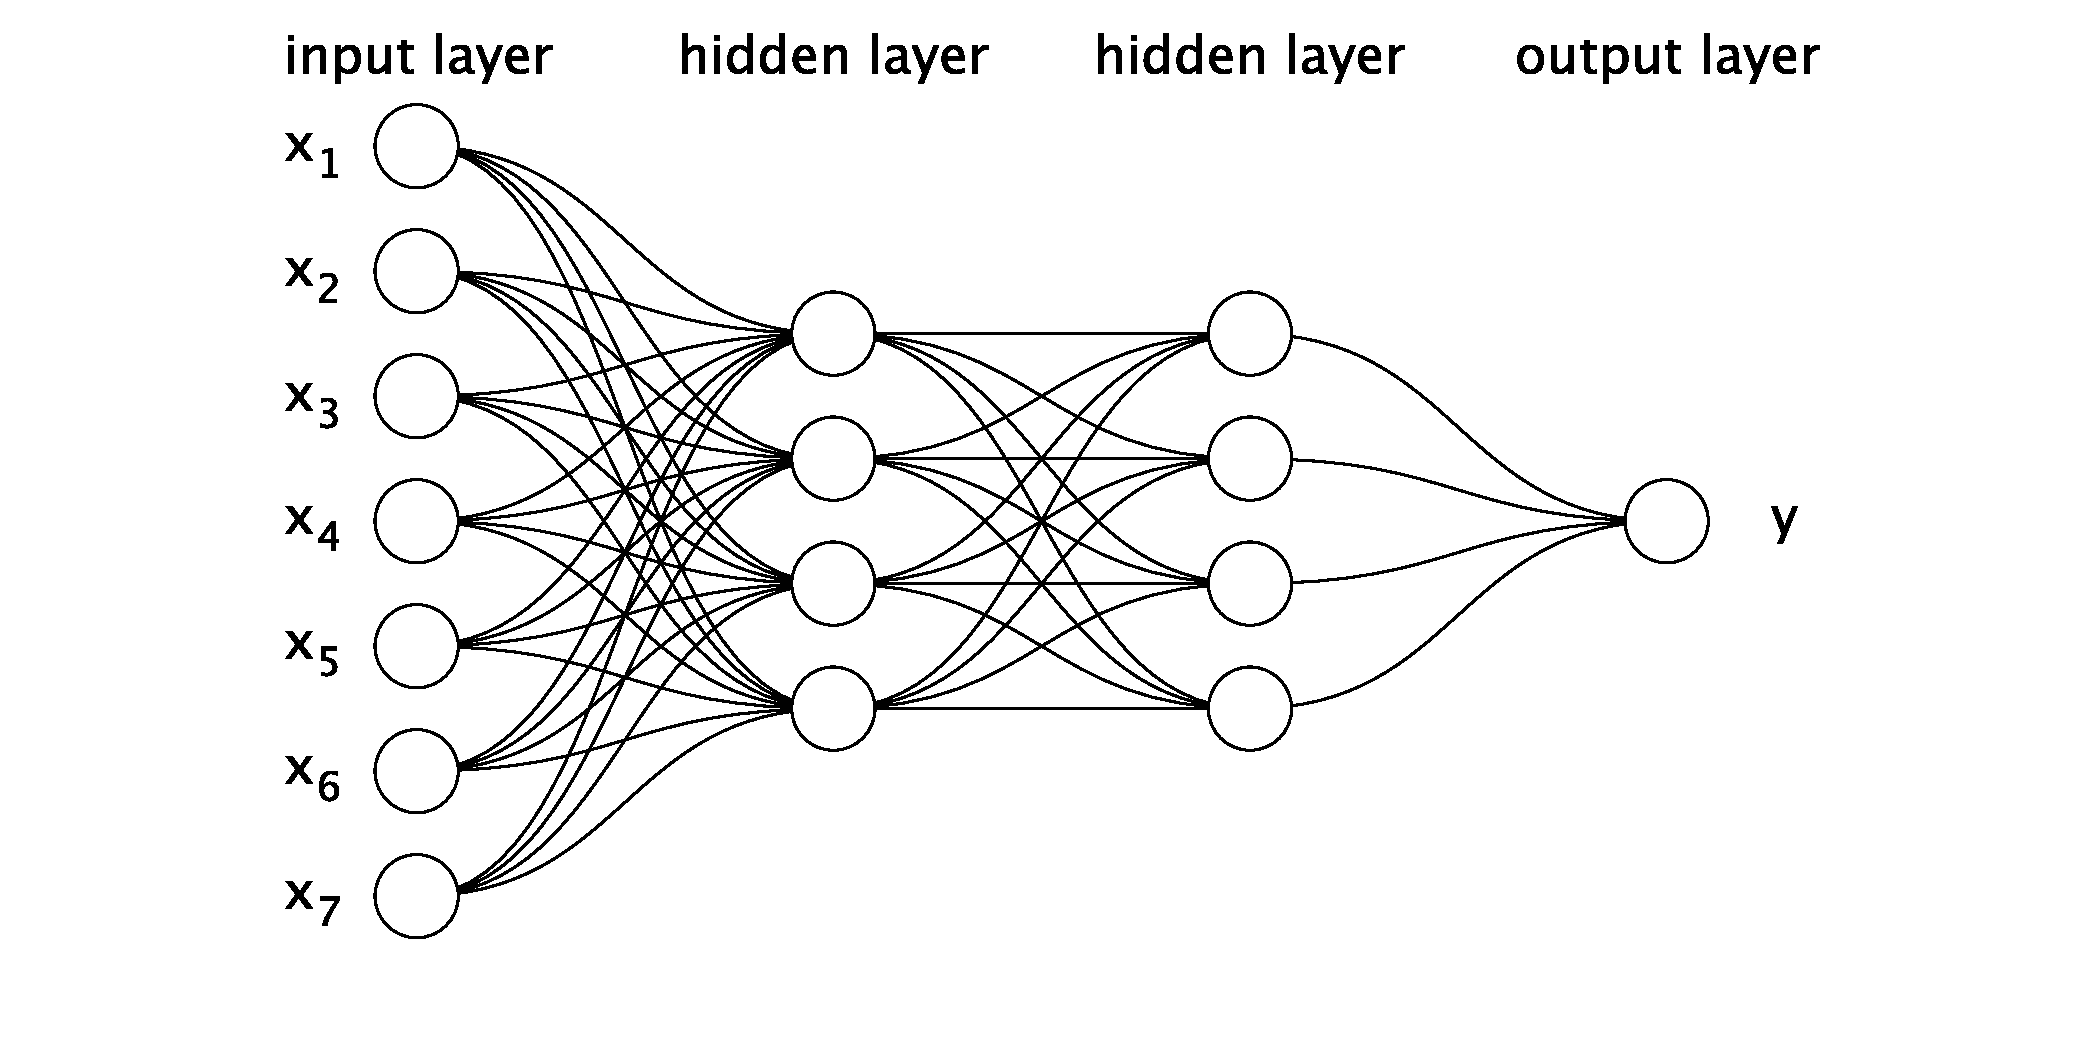
\includegraphics[width=1\textwidth]{examplenn.pdf}
 \caption{A neural network.}
 \label{examplenn}
\end{figure}

To understand the backpropagation algorithm, consider a network with only one output neuron (such as in Figure~\ref{examplenn}), and consider its prediction for a specific datapoint in the training set.
The squared error for this datapoint is \(\varepsilon = \left(y^\text{target} - y^\text{prediction}\right)^2\).
The target is fixed, and we cannot directly change the prediction, so to reduce \(\varepsilon\), we can calculate the change we need to make to each weight to reduce the error the most.
The prediction only depends on the outputs of the neurons on the previous layer and the weights connecting the layers.
This same logic applies to all of the neurons in the network.
Assuming that all the activation functions are differentiable, we can apply the chain rule repeatedly to calculate the gradient of the overall error with respect to each weight \(w_j\) in the network.
This gradient
\[ \Delta w_j = \diffp{\varepsilon(w_j)}{w_j} \]
represents the change needed to weight \(w_j\) to most steeply increase the error, so the value \(-\Delta w_j\) is the direction that most steeply decreases the error.
We scale this amount by a constant hyperparameter \(\eta\), called the \qt{learning rate}, and change each weight accordingly \(w_j = w_j - \eta \Delta w_j\).
We perform this process for each weight, and then for each datapoint in the training dataset.

This type of method is called \qt{stochastic gradient descent} (also called \qt{online gradient descent} or \qt{iterative gradient descent}) because it does not calculate the true steepest gradient.
Each datapoint moves the weights in a slightly different direction, so the optimisation process zigzags towards the optimum, rather than taking the steepest path.
An alternative is \qt{batch gradient descent}, where the sum of the squared errors for all the training data is calculated and optimised.
\[ \varepsilon(\vec{w}) = \frac{1}{2} \sum_{i}\left(y_i^\text{target} - y_i^\text{output}\right)^2 \]
This will converge to a solution in fewer steps, but takes significantly longer to compute.

Estimating the parameters of an \ac{ANN} using either type of gradient descent is guaranteed to find a local optimum given enough time, but is not guaranteed to converge to a global optimum.
It is quite rare for the algorithm to get trapped in a local minimum, but a more common problem is getting stuck at saddle points where the gradient is zero~\autocite[438]{lecun2015}.

\subsection{\citeauthor{minsky1987} and the \qt{AI winter}}

In 1969, \citeauthor{minsky1987} published \qt{Perceptrons}\footnote{Not to be confused with \qt{The Perceptron} by \textcite{rosenblatt1957}}, in which they described some of the limitations of Rosenblatt's perceptrons~\autocite{minsky1987}.
They admitted that the perceptron appears to be a powerful tool due to properties like the \qt{perceptron convergence theorem}, which states that for any linearly separable dataset, the perceptron classifier algorithm will find a solution in a finite number of steps.
However, their main criticism was that a perceptron could not solve linearly inseparable problems, which are problems where it is not possible to draw a single straight line, plane or hyperplane that correctly divides the points into their classes.

The example they used was the XOR function, defined as being true only when only one of its inputs is true (seen in Figure~\ref{xor}), which they proved was impossible for the perceptron to learn.

\begin{figure}[htbp]
 \centering
 \begin{subfigure}[t]{0.45\textwidth}
 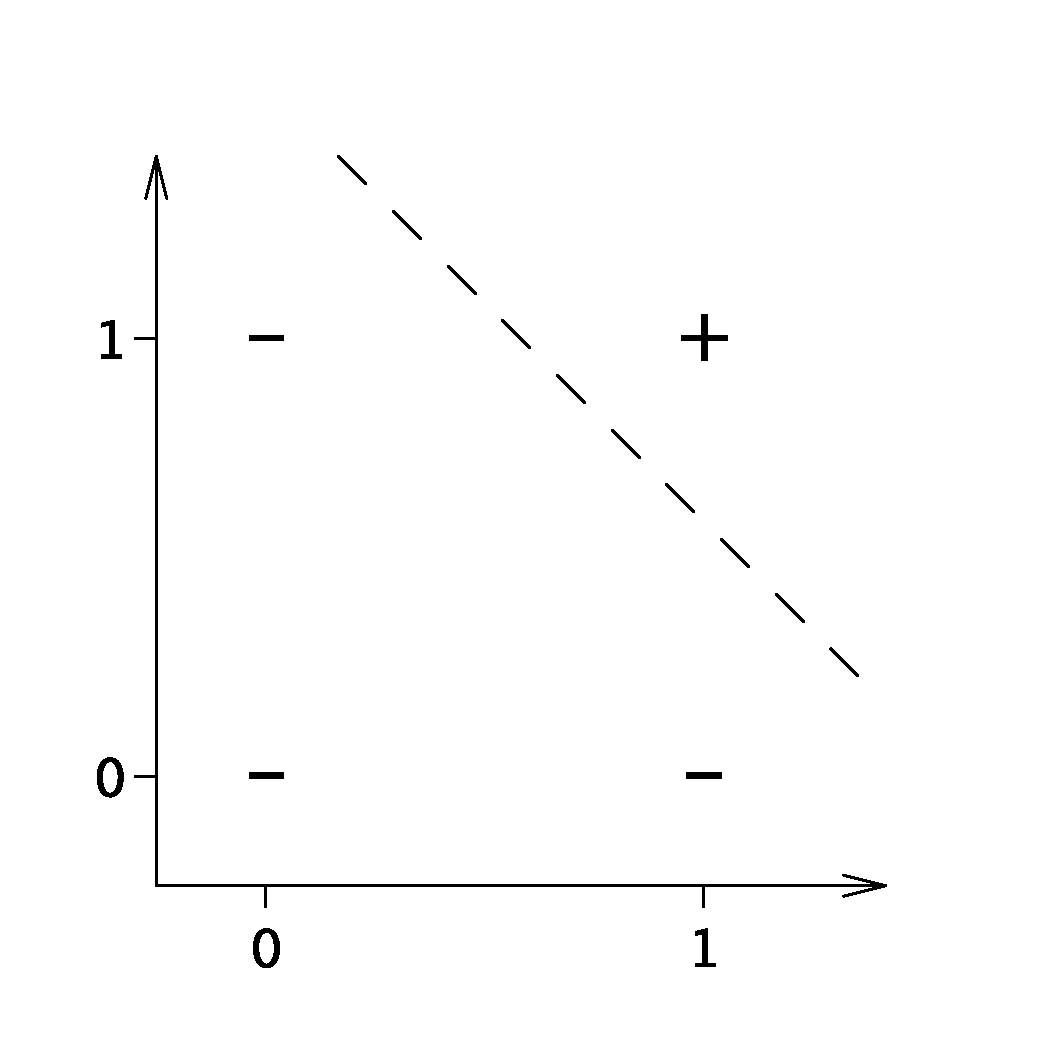
\includegraphics[width=\textwidth]{and.pdf}
 \caption{The AND function is linearly separable.}
 \label{and}
 \end{subfigure}
 ~ % horizontal space between subfigures
 \begin{subfigure}[t]{0.45\textwidth}
 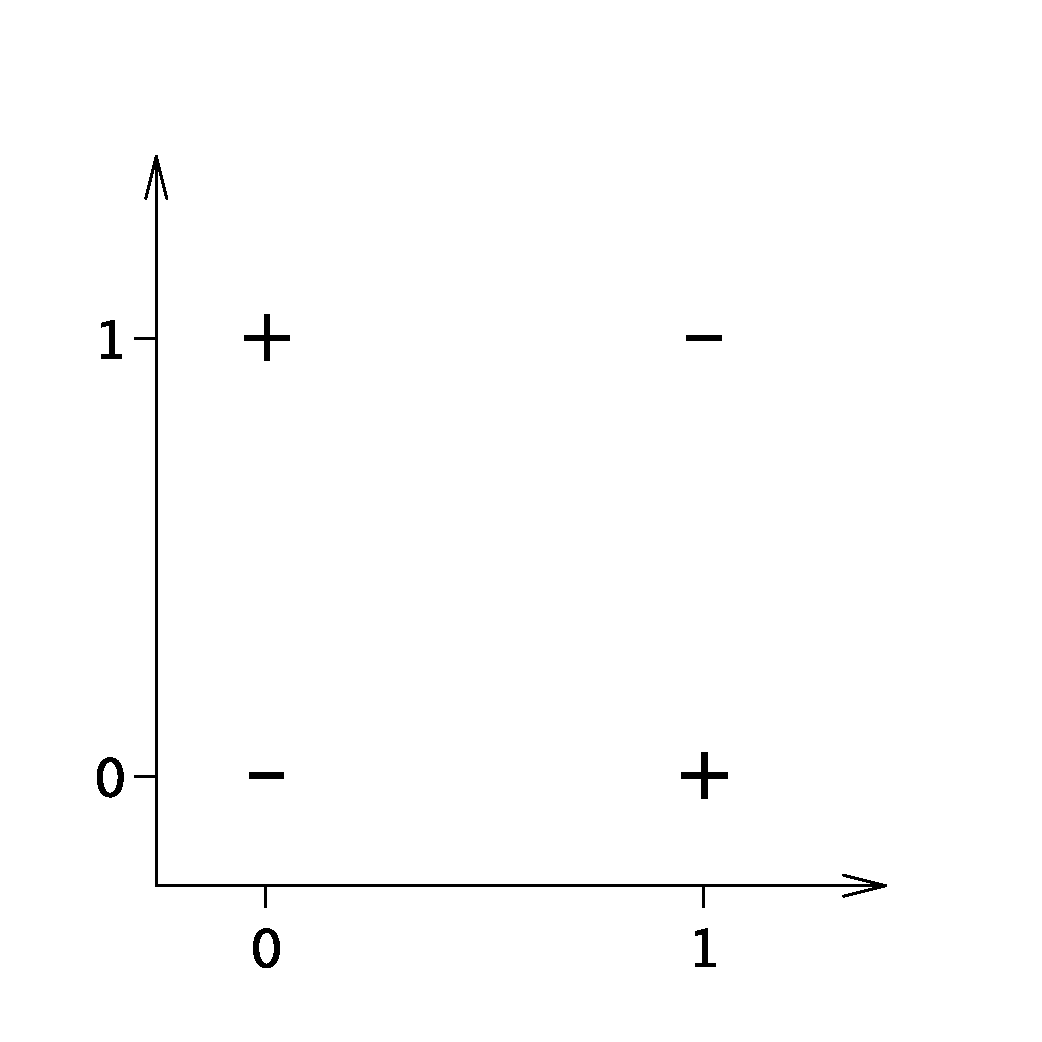
\includegraphics[width=\textwidth]{xor.pdf}
 \caption{The XOR function is not linearly separable.}
 \label{xor}
 \end{subfigure}
\caption{Two functions, the four possible input combinations and their outcomes. For the XOR function, there is no straight line that divides the two classes, so the XOR function is not linearly separable.}
\end{figure}

The biggest problem with \citeauthor{minsky1987}'s criticisms were that they only considered the \qt{simple perceptron}, a network with only one layer, and did not look at the possibility of multiple perceptrons being joined together~\autocite[514]{block1970}.
\citeauthor{minsky1987} seemed to misunderstand Rosenblatt's reasoning for developing the perceptron.
Their goal was to disprove the perceptron as a theory for the internals of the brain, however, Rosenblatt was more interested in recreating certain properties of a biological brain without regard for about the accuracy of the internal mechanisms~\autocite[516]{block1970}.
Despite the name of their book being \qt{Perceptrons}, they studied \qtc[517]{block1970}{a severely limited class of machines from a viewpoint quite alien to Rosenblatt's}.

As with many promising technologies, researchers working on perceptrons overpromised and underdelivered, causing a decline in interest and funding for the field.
For ML and \acp{ANN}, this period occurred in the 1970s, where other methods could produce similar results to a multilayer perceptron for the same or a much lower computing cost.
This period has been called the \qt{AI winter}.
The release of \qt{Perceptrons} is often blamed with causing this fallow period in funding for ML, but \citeauthor{minsky1987} claim that progress was already stagnant when they published their criticisms, and it would have occurred irrespective of their opinions.
With the revival of neural networks in the 1980s, it has been proposed that the severity of \citeauthor{minsky1987}'s criticisms as the cause of abandonment of \acp{ANN} was exaggerated to help legitimise alternative disciplines~\autocite[649]{olazaran1996}.

\subsection{Deep learning and the 21st century} \label{deeplearning}

As computing power has increased exponentially (following Moore's law), \acp{ANN} have become a more viable method of prediction.
In the 21st century, success has been found in increasing the number of layers in the network (depth) rather than the number of neurons in each layer (width).
These \qt{deep neural networks} \qtc[438]{lecun2015}{can implement extremely intricate functions of its inputs that are simultaneously sensitive to minute details}.
The ability of \ac{DL} algorithms to solve problems once thought impossible has caused a large amount of corporate interest, contrasting with the primarily academic interest when perceptrons were discovered.
\ac{DL} has even made its way into consumer products.
Many modern phones have facial recognition software built in, and \ac{AI} voice assistants are becoming more common in homes.
\ac{DL} is also becoming more accessible, with the release of Google's \qt{Tensorflow} package for \ac{DL}~\autocite{abadi2016}, which is now available in \qt{Keras}, a user friendly package for Python~\autocite{chollet2015} and R~\autocite{allaire2018}.
Given the amount of commercial success that \ac{DL} has seen, another AI winter seems unlikely.
